% ==========================
% # TV do \acrshort{deec}             #
% ==========================

\paragraph{TV do \acrshort{deec}}

O \acrshort{deec} tem televisões distribuídas pelo Departamento (nomeadamente no bar e na entrada do piso 2) onde é possível passar alguma informação nomeadamente notícias (em texto) e anúncios (em imagem). O \acrshort{neeec} costumava pedir à D. Ana Maria Bernardes para colocar informação (em texto) nestas televisões de forma a publicitar os seus eventos. Este processo repetia-se para as atividades de maior dimensão apenas. Após conversações com o GRI, o \acrshort{neeec} passou a ter uma conta de acesso à plataforma que permite a inserção dos dados nas televisões (http://cptv.streamline.pt/\#/login) passando, desta forma, o \acrshort{neeec} a fazer também a gestão da televisão. Adicionalmente, o \acrshort{neeec} incentivou o \acrshort{gri} a criar uma nova funcionalidade na plataforma que permite a inserção de imagens (1040 x 840 pixeis) passando assim a ser possível inserir imagens como se pode ver na figura \ref{fig:tvDEEC1}.

\begin{figure}[ht]
\centering
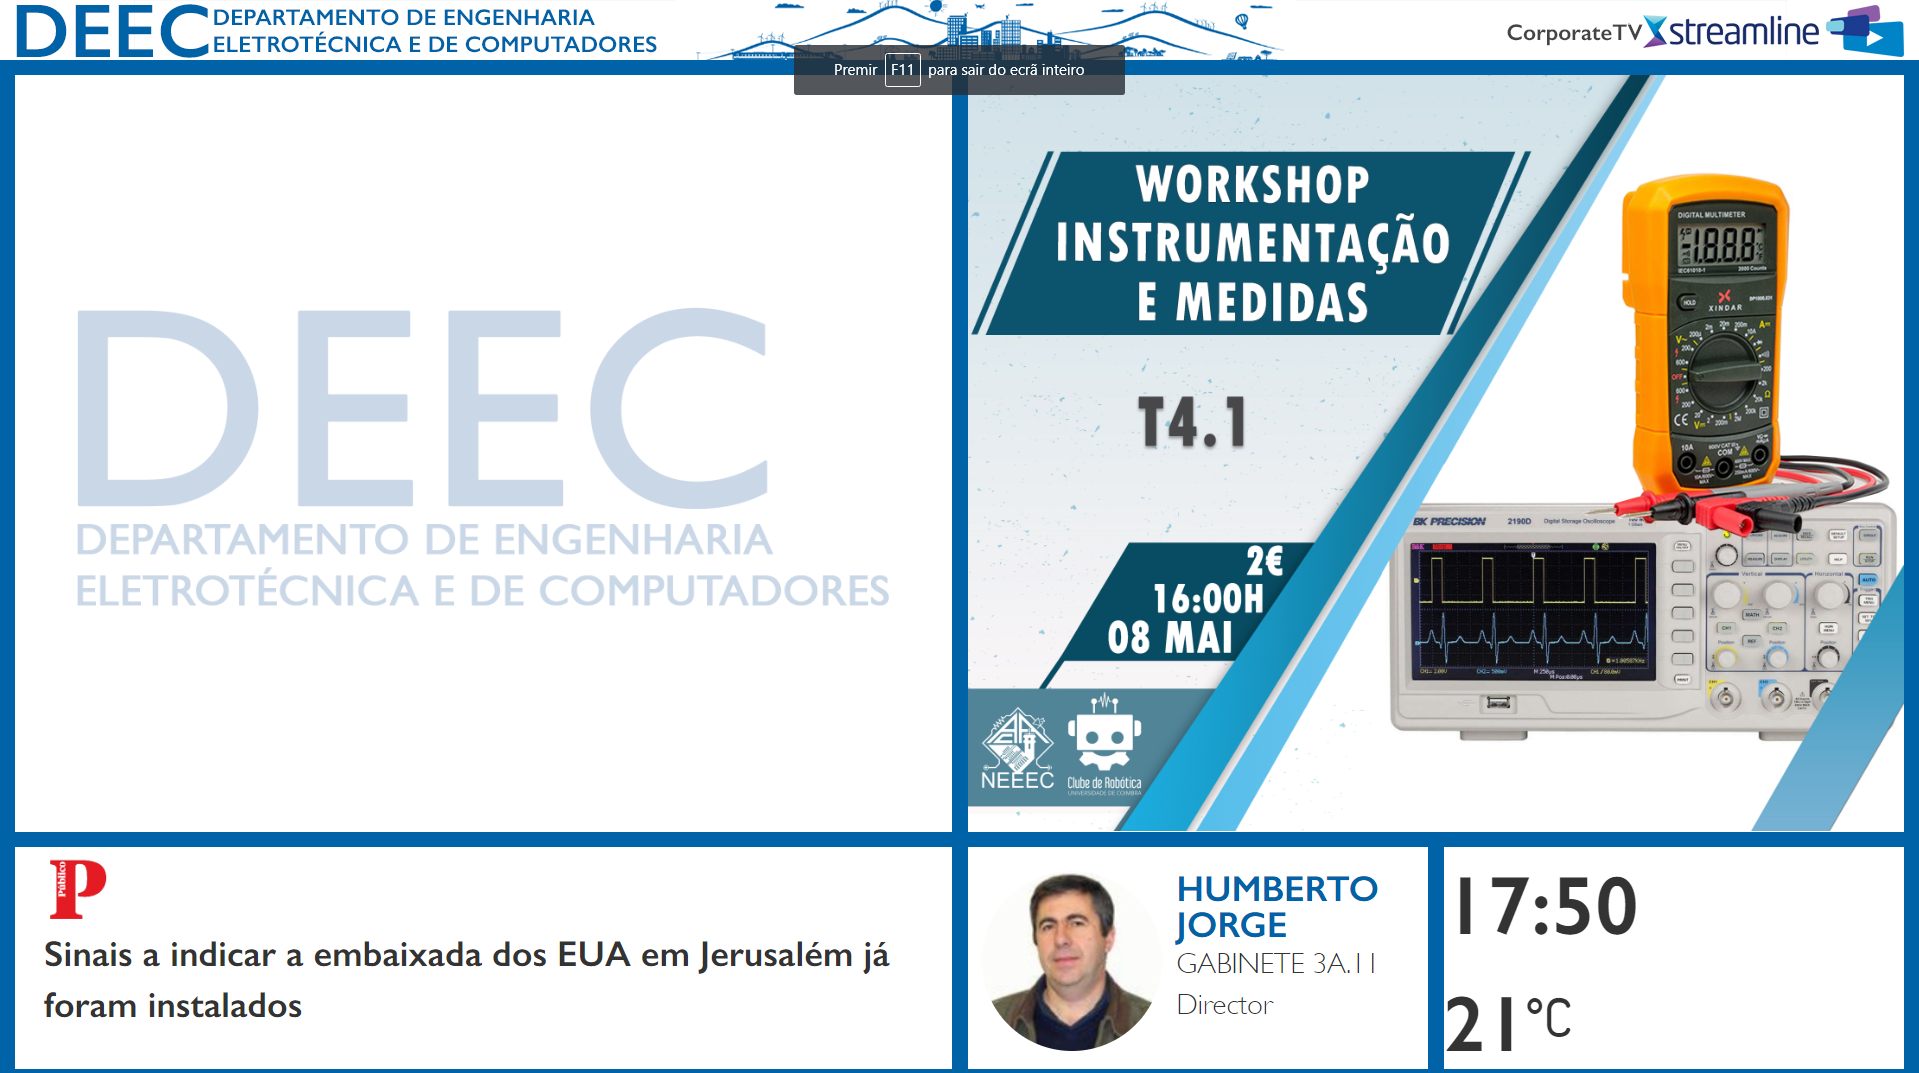
\includegraphics[width=\textwidth]{imagens/tvDEEC1.png}
\caption{Layout antigo.}
\label{fig:tvDEEC1}
\end{figure}

Adicionalmente, após umas obras de remodelação da sala de reuniões do \acrshort{deec}, o professor Humberto Jorge ofereceu uma televisão ao \acrshort{neeec}. Esta televisão foi instalada na sala de convívio tendo também sido instalado um pc que permite a exibição do layout das tv’s do \acrshort{deec} nesse ecrã. O GRI, gentilmente, criou um novo layout específico para o \acrshort{neeec} que ficou em exibição nessa televisão e pode ser visto na figure \ref{fig:tvDEEC2}.

\begin{figure}[ht]
\centering
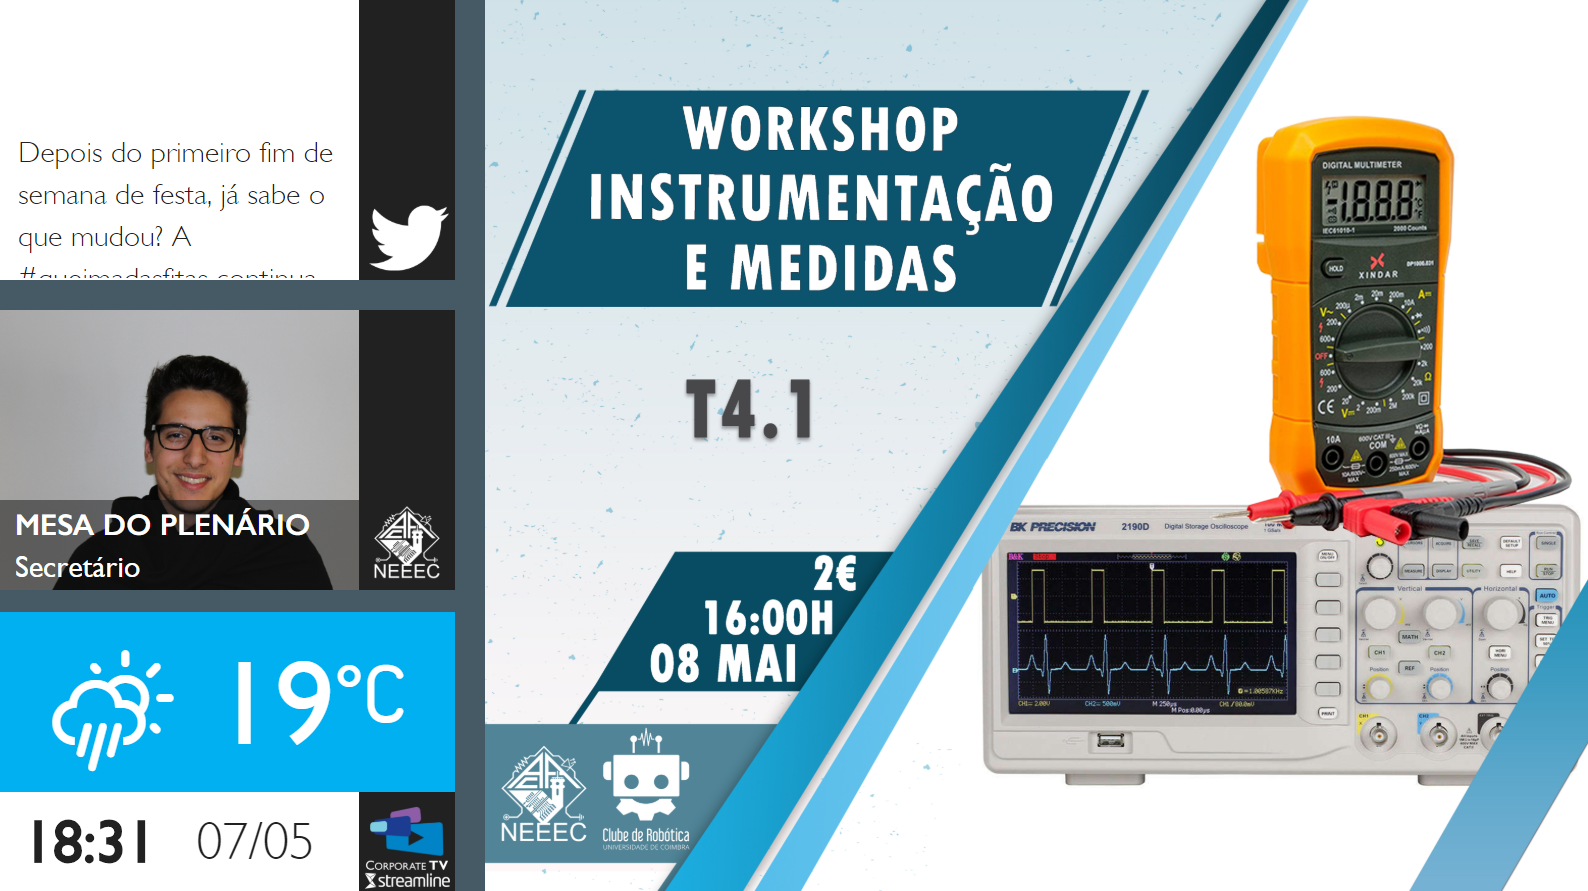
\includegraphics[width=\textwidth]{imagens/tvDEEC2.png}
\caption{Layout criado para o \acrshort{neeec}.}
\label{fig:tvDEEC2}
\end{figure}

Todos os layouts são totalmente configuráveis na plataforma onde se inserem as imagens. As fotos, nomes e cargos dos membros do \acrshort{neeec} que aparecem na tv, podem ser alterados através de um ficheiro que se encontra no servidor onde está alojado o site do \acrshort{neeec}.

\begin{itemize}
\item Inserir imagens/notícias na plataforma:
	\begin{itemize}
	\item Aceder a http://cptv.streamline.pt/\#/login;
    \item Selecionar o ícone de editar ao lado de \acrshort{fctuc} | Departamento de Eng. Eletrónica e de Computadores;
    \item Descer até à secção de imagens e clicar em “Upload de imagens”;
    \item Escolher o(s) ficheiro(s) a enviar;
    \item Ir à galeria de imagens, selecionar a foto que se pretende colocar na notícia e pressionar em “Copiar URL”;
    \item Selecionar “Voltar à edição” e ir à área de notícias, selecionando o ícone do balão de fala para adicionar uma nova notícia;
    \item Caso se pretenda inserir apenas uma imagem, selecionar, no tipo, “Imagem” e colar o URL da imagem no campo devido. Colocar um título na notícia (não irá ser mostrado);
    \item Escolher a data (após a data selecionada como data de fim a notícia irá deixar de estar visível nas televisões);
    \item Carregar em alterar;
    \item Para inserir uma notícia de texto basta, no tipo, selecionar “Informação”. Neste modo é também possível inserir imagens devendo-se proceder da mesma forma para copiar o URL da imagem. Deve-se depois, no campo “Conteúdo”, selecionar o ícone de imagem e colocar a foto que se pretende, dimensionando também o tamanho e escolhendo a posição da imagem no ecrã.
	\end{itemize}
\end{itemize}

Este meio veio facilitar o nosso trabalho por permite a inserção de textos, vídeos e imagens com uma data de início e uma data de fim de divulgação que poderá ser posterior à atual. Desta forma, a imagem ao criar a imagem dos eventos enviava sempre uma imagem para o formato da tv sendo assim possível inseri-la no sistema e ter mais um meio de divulgação que funciona bastante bem, de forma fácil, uma vez que é tem uma divulgação dinâmica e está sempre organizado de forma automática.